%
% Appendix C.- About Quotes and Photos
%
% Resize and cut 826 x 413
% Filter
%     Artistic -> GIMPressionist -> Dotify
% Colors
%     Colorize -> (H,S,L): (24, 84, 10)
%                                  (0.06, 0.84, 0.1)  

\chapterimage{ouroboros.pdf} % Chapter heading image

\chapter{About Quotes and Photos}
\label{apx:photos}

\begin{quote}
\begin{flushright}
\emph{What we know is little, \\
combined with tenacious concentration on a subject\\
and what we are ignorant of is immense.}\\
Pierre-Simon Laplace
\end{flushright}
\end{quote}
\bigskip

This appendix gathers the quotes and photographs that appear at the beginning of each chapter, offering a brief explanation of their origin and meaning. These elements were carefully chosen for their deep symbolic connection to the central themes of the theory of nescience. The quotations capture, in a few words, timeless insights about knowledge, ignorance, discovery, and the creative power of questioning; some of them serving as true sources of inspiration in the development of the theory itself.

The photographs, likewise, are not mere illustrations: each has been selected as a visual metaphor for a key concept discussed in the book, and has been pre-processed to ensure a coherent visual style. Together, these quotes and images form a symbolic framework that accompanies the reader throughout the book, signposting the intellectual journey from the unknown to the known.

%
% Section: About Quotes
%

\section{Chapter Quotes}

The quotations collected in the book have been carefully selected for their profound relevance to the theory of nescience. Each captures, in a few words, a key idea about knowledge, ignorance, discovery, or the creative act of questioning, all central to the themes explored throughout this book. Some of these quotes have been a genuine source of inspiration in the development of the theory itself, shaping its concepts and guiding its spirit. They are presented here as intellectual signposts, inviting the reader to reflect on the timeless wisdom that underlies our ongoing quest to illuminate the unknown.

\vspace{1em}

\noindent
\textquotedblleft Perfection is achieved not when there is nothing more to add, but when there is nothing left to take away.\textquotedblright \\
\emph{Antoine de Saint-Exupéry} \\
French aviator and author of \emph{The Little Prince}, Saint-Exupéry combined technical discipline with poetic clarity. This quote celebrates the art of refinement: true perfection emerges not from accumulation, but from stripping away the superfluous to reveal the essential. It resonates with the theory of nescience, which seeks to reduce surfeit, eliminating redundant information until only the irreducible core of knowledge remains.

\vspace{1em}

\noindent
\textquotedblleft If presented with a choice between indifferent alternatives, then one ought to select the simplest one.\textquotedblright \\
\emph{William of Ockham (Occam's Razor)} \\
The medieval philosopher William of Ockham championed conceptual economy in an age of scholastic excess. His Razor urges us to prefer simplicity when multiple explanations fit the same evidence. This principle aligns with nescience by warning against needless complexity, guiding us to seek the most compact and accurate representations of knowledge.

\vspace{1em}

\noindent
\textquotedblleft We are all agreed that your theory is crazy. The question which divides us is whether it is crazy enough.\textquotedblright \\
\emph{Niels Bohr} \\
Bohr, a founder of quantum theory, embraced the paradoxes that reshaped modern physics. His quip reminds us that revolutionary ideas often seem absurd at first. It underscores the need for bold conceptual leaps to break through entrenched assumptions and reveal what lies hidden in the unknown.

\vspace{1em}

\noindent
\textquotedblleft All great work is the fruit of patience and perseverance, combined with tenacious concentration on a subject over a period of months or years.\textquotedblright \\
\emph{Santiago Ramón y Cajal} \\
The father of modern neuroscience, Ramón y Cajal spent decades meticulously mapping the nervous system. His words highlight the slow, deliberate nature of deep discovery. For nescience, they affirm that overcoming ignorance is rarely sudden; it demands sustained, focused engagement with the unknown.

\vspace{1em}

\noindent
\textquotedblleft A little inaccuracy sometimes saves tons of explanation.\textquotedblright \\
\emph{Saki (H. H. Munro)} \\
Known for his concise, satirical stories, Saki understood the power of brevity. This remark suggests that relentless precision can hinder clarity, and that small simplifications can reveal the bigger picture. It speaks to nescience by acknowledging that small sacrifices in exactness can accelerate the broader reduction of ignorance.

\vspace{1em}

\noindent
\textquotedblleft Everything should be made as simple as possible, but not simpler.\textquotedblright \\
\emph{Albert Einstein} \\
Einstein revolutionized physics through elegant, minimalist theories, yet he warned against oversimplification. His maxim captures the delicate balance at the heart of nescience: reducing the length and complexity of our descriptions without introducing errors that distort reality.

\vspace{1em}

\noindent
\textquotedblleft There are known knowns\ldots\ There are things we don't know we don't know.\textquotedblright \\
\emph{Donald Rumsfeld} \\
Though a political figure, Rumsfeld articulated a taxonomy of knowledge that became famous beyond its context. He distinguished what we know, what we know we don't know, and what we don't even realize we don't know. This hierarchy mirrors the structure of nescience, which measures progress by transforming unknown unknowns into known unknowns, and eventually into knowns.

\vspace{1em}

\noindent
\textquotedblleft It is not the answer that enlightens, but the question.\textquotedblright \\
\emph{Eugène Ionesco} \\
A pioneer of the Theatre of the Absurd, Ionesco used paradox to challenge conventional thinking. His statement celebrates the generative power of questions, which open new conceptual spaces. Nescience places similar emphasis on asking fruitful questions as the first step toward uncovering the hidden unknown.

\vspace{1em}

\noindent
\textquotedblleft There are no difficult problems, only lack of imagination.\textquotedblright \\
\emph{Antonio García} \\
A Spanish engineer, García championed creativity as the key to problem-solving. His observation reframes obstacles as failures of perspective rather than inherent difficulty. This spirit of imaginative thinking is vital to finding new ways to approach what seems unknowable.

\vspace{1em}

\noindent
\textquotedblleft Science may be regarded as the art of data compression.\textquotedblright \\
\emph{Ming Li \& Paul Vitányi} \\
Pioneers of algorithmic information theory, Li and Vitányi showed that scientific theories compress vast datasets into concise descriptions. Their insight directly underpins science: progress is measured by how much shorter and more accurate our descriptions become as we transform scattered facts into structured knowledge.

\vspace{1em}

\noindent
\textquotedblleft To be surprised, to wonder, is to begin to understand.\textquotedblright \\
\emph{José Ortega y Gasset} \\
A leading Spanish philosopher, Ortega y Gasset saw wonder as the spark of understanding. This quote marks the moment when the familiar becomes strange enough to question. That moment, recognizing something as unknown, is the first step in reducing it.

\vspace{1em}

\noindent
\textquotedblleft Mathematics may be defined as the subject in which we never know what we are talking about, nor whether what we are saying is true.\textquotedblright \\
\emph{Bertrand Russell} \\
Logician, philosopher, and Nobel laureate, Russell used humor to reveal the abstract nature of mathematics. His quip highlights how mathematical structures often float free of meaning. This echoes nescience's concern that our representations may be precise yet disconnected from reality, requiring continual testing to ground them.

\vspace{1em}

\noindent
\textquotedblleft The purpose of models is not to fit the data but to sharpen the questions.\textquotedblright \\
\emph{Samuel Karlin} \\
Karlin, a mathematician who bridged probability and biology, valued models as tools for inquiry. His statement reframes models not as answers but as catalysts for better questions. This perspective resonates with science, where models are judged not just by accuracy but by how they illuminate unexplored unknowns.

\vspace{1em}

\noindent
\textquotedblleft Wanderer, there is no road; the road is made by walking.\textquotedblright \\
\emph{Antonio Machado} \\
One of Spain's most beloved poets, Machado captured the spirit of exploration. His verse suggests that progress comes from forging paths rather than following them. Reducing ignorance often means inventing entirely new conceptual routes through uncharted intellectual terrain.

\vspace{1em}

\noindent
\textquotedblleft Information is the resolution of uncertainty.\textquotedblright \\
\emph{Claude Shannon} \\
The father of information theory, Shannon redefined knowledge as the reduction of uncertainty. This precise definition transformed communication and computing. It also aligns perfectly with nescience, which measures discovery by how much it reduces inaccuracy and brings clarity to the unknown.

\vspace{1em}

\noindent
\textquotedblleft An approximate answer to the right problem is worth a good deal more than an exact answer to an approximate problem.\textquotedblright \\
\emph{John Tukey} \\
A trailblazing statistician, Tukey emphasized exploratory thinking over rote analysis. His maxim warns that asking the wrong question wastes precision. It affirms that choosing the right unknown to explore matters more than perfectly solving a trivial one.

\vspace{1em}

\noindent
\textquotedblleft Some mathematical statements are true for no reason; they're true by accident.\textquotedblright \\
\emph{Gregory Chaitin} \\
Chaitin, a founder of algorithmic information theory, exposed the limits of provability. His remark highlights that some truths are irreducible and beyond explanation. This insight sets a boundary for science: not all unknowns can be conquered, some are unknowable by nature.

\vspace{1em}

\noindent
\textquotedblleft To go where you don't know, you have to go by a way you don't know.\textquotedblright \\
\emph{Saint John of the Cross} \\
The Spanish mystic and poet portrayed spiritual growth as a journey through darkness. This line captures the essence of venturing beyond the familiar. Reaching the unknown unknown requires abandoning well-worn methods and daring to step into paths yet unimagined.

%
% Section: About the Photos
%

\section{Chapter Pitures}

The photographs presented at the beginning of each chapter have been carefully selected for their symbolic significance and their deep connection to the central themes of the theory of nescience. Each image embodies a key idea explored in the book, such as the pursuit of knowledge, the struggle against ignorance, the propagation of understanding across generations, and the continual expansion of the frontiers of the known. Rather than serving as mere decoration, these images act as visual metaphors, inviting the reader to reflect on the broader meaning of the concepts discussed in each chapter.

All the photographs included here are believed to be royalty-free (or at least publicly usable according to their appearance on Google Images). In addition, every image has been pre-processed using GIMP\footnote{\url{http://www.gimp.org}}, the GNU Image Manipulation Program, to enhance their clarity, contrast, and compositional balance, ensuring a consistent visual style throughout the book. This curated selection aims to enrich the reading experience, providing a visual narrative that parallels the intellectual journey from ignorance to understanding.

\subsubsection* {The Torch Bearers}

\begin{wrapfigure}{L}{0.3\textwidth}
\centering
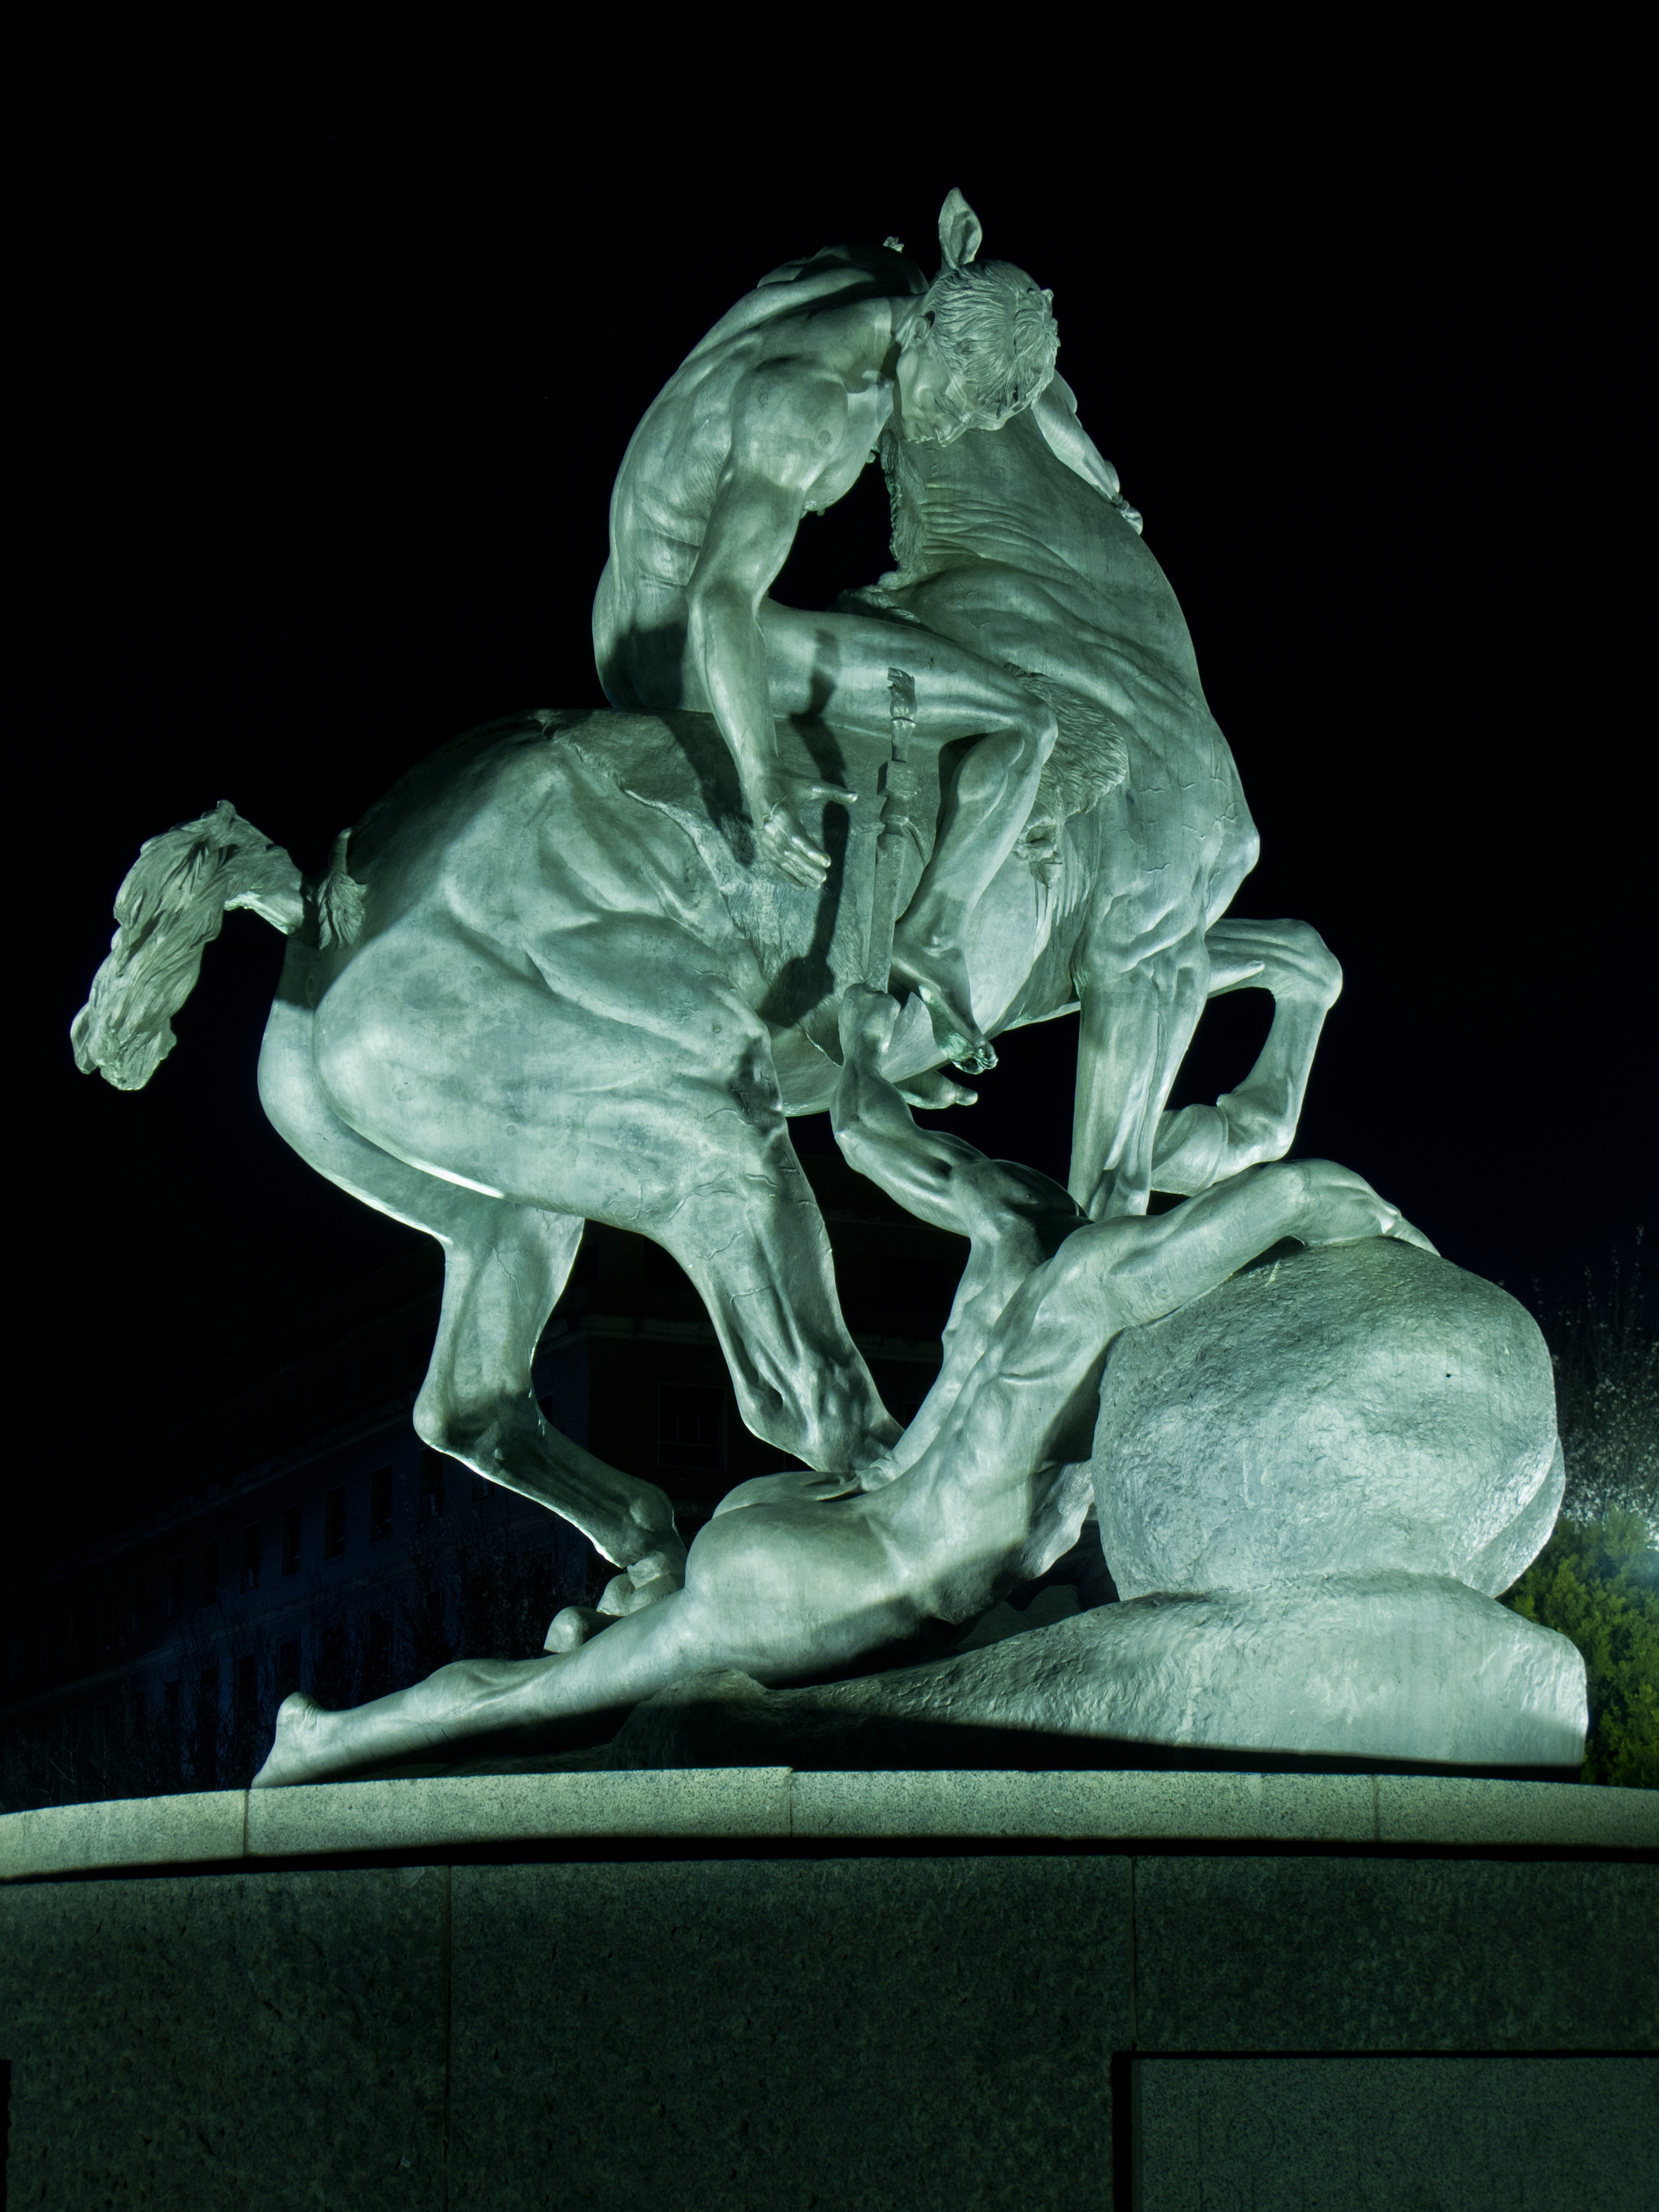
\includegraphics[width=0.15\textwidth]{Los_portadores_de_la_antorcha_-_05.pdf}
\end{wrapfigure}

The Torch Bearers is an aluminum sculpture by the American artist Anna Hyatt Huntington, donated to the city of Madrid in 1955 and now located on the campus of the Universidad Complutense. The work depicts an old, dying man passing a flaming torch to a vigorous young rider, who carries it forward with determination. The torch symbolizes the light of knowledge, handed from one generation to the next in humanity's endless pursuit of understanding. As each generation advances the frontier of the known, they also illuminate new regions of the unknown, leaving an enduring legacy for their successors to explore. Huntington also created bronze casts of the sculpture, which can be found in Valencia, Havana, and at several cultural institutions across the United States.

\subsubsection* {The Allegory of the Cave}

\begin{wrapfigure}{L}{0.3\textwidth}
\centering
\includegraphics[width=0.30\textwidth]{Platonic_cave.pdf}
\end{wrapfigure}

The Allegory of the Cave, conceived by the Greek philosopher Plato, illustrates humanity's struggle to move from illusion to understanding. Prisoners are chained in a cave, able to see only shadows cast on a wall, mistaking these fleeting silhouettes for reality. When one prisoner breaks free and ascends to the surface, he is at first blinded by the light, but gradually perceives the true forms of things under the sun. This image embodies the essence of the theory of nescience: our initial grasp of the world is partial and distorted, yet through effort, questioning, and discovery we can escape the cave of ignorance and illuminate what was once unknown.

\newpage

\subsubsection* {Ars Magna}

\begin{wrapfigure}{L}{0.3\textwidth}
\centering
\includegraphics[width=0.30\textwidth]{Ramon_Llull_-_Ars_Magna_Fig_1.pdf}
\end{wrapfigure}

Ars Generalis Ultima, also known as the Ars Magna ("The Ultimate General Art"), was a groundbreaking work published in 1305 by the Spanish philosopher Ramon Llull. In it, Llull described a mechanical method for reasoning, composed of concentric rotating wheels inscribed with fundamental concepts. By systematically combining these elements, the device aimed to generate all possible logical truths about a given topic (especially to defend and explain Christian beliefs through rational argument). Although primitive by modern standards, Llull's invention represents one of the earliest attempts to use formal logic as a tool for discovery. It stands as a distant ancestor of modern computational thinking and an early expression of the human desire to reduce ignorance by unveiling hidden relations between ideas.

\subsubsection* {Galileo's Telescope}

\begin{wrapfigure}{L}{0.3\textwidth}
\centering
\includegraphics[width=0.30\textwidth]{Galileos-telescope-002.pdf}
\end{wrapfigure}

Galileo Galilei was an Italian astronomer, physicist, engineer, philosopher, and mathematician who helped ignite the scientific revolution of the seventeenth century. He was among the first to proclaim that the language of nature is written in mathematics, and that its laws can be unveiled through systematic observation and reasoning. In 1610, Galileo built a telescope and turned it toward the heavens, revealing mountains on the Moon, the moons of Jupiter, and countless stars invisible to the naked eye. These discoveries shattered long-held beliefs and expanded the boundaries of the known cosmos. His telescope thus became a symbol of humanity's enduring drive to pierce the veil of ignorance.

\subsubsection* {Athena's Owl}

\begin{wrapfigure}{L}{0.3\textwidth}
\centering
\includegraphics[width=0.30\textwidth]{owl.pdf}
\end{wrapfigure}

This ancient silver coin depicts the owl of Athena, the Greek goddess of wisdom. Revered as a symbol of knowledge, insight, and scholarly pursuit throughout the Western tradition, the owl embodies the capacity to see through darkness, just as understanding allows us to pierce the unknown. The German philosopher Hegel famously wrote that "the owl of Athena spreads its wings only with the falling of the dusk," suggesting that philosophy comprehends the meaning of an era only as it fades into the past. In this sense, the owl reminds us that knowledge often arrives after the fact, illuminating what once was obscure.

\subsubsection* {Escher's Infinite Stairs}

\begin{wrapfigure}{L}{0.3\textwidth}
\centering
\includegraphics[width=0.30\textwidth]{Escher.pdf}
\end{wrapfigure}

This artwork, known as "Relativity" by M. C. Escher, depicts figures endlessly walking along staircases that defy the laws of geometry and gravity. Each group of figures moves consistently within its own frame of reference, yet the perspectives are incompatible with one another, creating an impossible structure. This paradoxical scene symbolizes the essence of miscoding: when our representations of reality are flawed, they can lead to coherent but fundamentally incorrect interpretations. Like the figures trapped in Escher's world, we may continue along logical paths that never converge on truth, illustrating how mistaken encodings can imprison thought within self-consistent illusions, a central concern in the theory of nescience.

\subsubsection* {Train Wreck at Montparnasse}

\begin{wrapfigure}{L}{0.3\textwidth}
\centering
\includegraphics[width=0.30\textwidth]{Train_wreck_at_Montparnasse_1895.pdf}
\end{wrapfigure}

This historic photograph captures the train wreck at Montparnasse Station in Paris in 1895, when an express locomotive overran the buffer stop, crashed through the station wall, and plunged onto the street below. The accident, caused by a combination of mechanical failure and human miscalculation, serves as a striking metaphor for inaccuracy. Even small errors in the models we use to predict and control complex systems can propagate into catastrophic failures when reality does not behave as expected. This image reminds us that inaccurate descriptions of the world not only mislead our understanding but can also derail our reasoning, sometimes with dramatic consequences.

\subsubsection* {Alexander Cuts the Gordian Knot}

\begin{wrapfigure}{L}{0.3\textwidth}
\centering
\includegraphics[width=0.30\textwidth]{Alexander_cuts_the_Gordian_Knot.pdf}
\end{wrapfigure}

This painting depicts the legendary moment when Alexander the Great confronted the Gordian Knot, an impossibly tangled cord tied to an ancient chariot in the city of Gordium. According to prophecy, whoever could untie the knot would become ruler of Asia. Rather than struggling to unravel its countless coils, Alexander drew his sword and cut through it in a single stroke. This bold act symbolizes the triumph of simplicity over unnecessary complexity, an apt metaphor for surfeit, the burden of excessive and redundant information that obscures true understanding. This image reminds us that insight often comes not from adding more complexity, but from daring to strip it away to reveal the underlying essence of a problem.

\newpage

\subsubsection* {Creation of Adam}

\begin{wrapfigure}{L}{0.3\textwidth}
\centering
\includegraphics[width=0.30\textwidth]{Creation_of_Adam.pdf}
\end{wrapfigure}

This detail from Michelangelo's The Creation of Adam, painted on the ceiling of the Sistine Chapel, captures the moment when the hand of God reaches out to spark life, and with it, the potential for knowledge, into humanity. The near-touching fingers symbolize the latent connection between the divine source of truth and the human capacity to grasp it. This image embodies the idea that all knowledge exists in principle, yet remains inaccessible until we reach for it. What separates ignorance from understanding is the daring act of extending our minds toward the unknown, bridging the gap between what is given and what is comprehended.

\subsubsection* {Rodin's The Thinker}

\begin{wrapfigure}{L}{0.3\textwidth}
\centering
\includegraphics[width=0.30\textwidth]{thinker.pdf}
\end{wrapfigure}

This sculpture, The Thinker by Auguste Rodin, portrays a solitary figure immersed in deep contemplation, his entire body tense with the effort of thought. Far from passive, his posture reveals thinking as an act of creation, shaping new possibilities within the mind. This image symbolizes the vital activity of discovering interesting questions: reaching beyond what is known, probing the boundaries of understanding, and daring to imagine what has not yet been asked. Every breakthrough begins not with an answer, but with the courage to pose a question that opens a new path into the unknown.

\subsubsection* {Rossum's Universal Robots}

\begin{wrapfigure}{L}{0.3\textwidth}
\centering
\includegraphics[width=0.30\textwidth]{Capek_play.pdf}
\end{wrapfigure}

This photograph shows a scene from R.U.R. (Rossum's Universal Robots), the 1920 play by Karel Čapek that introduced the word robot to the world. In the play, artificial beings are created to perform human labor, eventually surpassing their makers. This early vision of automation resonates with the modern ambition of machine learning: building systems capable of discovering patterns and generating knowledge with minimal human intervention. The image symbolizes the quest to construct machines that can autonomously reduce our ignorance, relentlessly searching through the unknown to uncover new truths, guided by the principle of minimizing nescience.

\newpage

\subsubsection* {Large Hadron Collider}

\begin{wrapfigure}{L}{0.3\textwidth}
\centering
\includegraphics[width=0.30\textwidth]{LHC.pdf}
\end{wrapfigure}

This image shows the traces of particles produced in a collision inside the Large Hadron Collider (LHC) at CERN, where protons are accelerated to near-light speeds and smashed together to probe the fundamental structure of matter. Each collision generates a burst of data that allows scientists to test hypotheses, refine theories, and discard false models. This process vividly illustrates how research reduces ignorance: by confronting the unknown through controlled experimentation, science transforms uncertainty into knowledge. Such experiments provide measurable evidence of progress, as each discovery narrows the gap between what is known and what remains to be uncovered.

\subsubsection* {Wikipedia Monument}

\begin{wrapfigure}{L}{0.3\textwidth}
\centering
\includegraphics[width=0.30\textwidth]{Wikipedia_Monument_2.pdf}
\end{wrapfigure}

The Wikipedia Monument, located in Słubice, Poland, was created by the Armenian sculptor Mihran Hakobyan and unveiled in October 2014 as the world's first monument dedicated to the online encyclopedia. The statue honors the countless anonymous editors who, across all cultures and languages, have voluntarily contributed to building one of humanity's most ambitious collective knowledge projects. The inscription celebrates Wikipedia as a symbol of global collaboration beyond political, religious, and cultural boundaries. A foundation for a knowledge society capable of fostering sustainable development, social justice, and peace among nations. This monument stands as a testament to the creative power of many minds working together to illuminate the unknown, piece by piece, like assembling the fragments of an ever-expanding puzzle.

\subsubsection* {Königsberg Bridges}

\begin{wrapfigure}{L}{0.3\textwidth}
\centering
\includegraphics[width=0.30\textwidth]{Koenigsberg_Map_by_Bering_1613.pdf}
\end{wrapfigure}

The old city of Königsberg in Prussia (now Kaliningrad, Russia) was built on both banks of the Pregel River, with two large islands linked to each other and to the mainland by seven bridges. The famous Seven Bridges of Königsberg problem asked whether it was possible to devise a walk that crossed each bridge exactly once, starting and ending at any point. In 1736, the Swiss mathematician Leonhard Euler proved that such a walk was impossible. His elegant solution marked the birth of graph theory, a new branch of mathematics that studies the structure of connections, a foundational concept in discrete mathematics and in the formal representation of knowledge.

\subsubsection* {Galton's Box}

\begin{wrapfigure}{L}{0.3\textwidth}
\centering
\includegraphics[width=0.30\textwidth]{Galton_box}
\end{wrapfigure}

This device, known as a Galton box or quincunx, was invented by the English scientist Francis Galton to demonstrate the principles of probability and the emergence of statistical regularities. Small balls dropped from the top bounce randomly off a series of pegs, eventually accumulating in bins at the bottom to form the familiar bell-shaped curve of the normal distribution. Although each individual path is unpredictable, the collective outcome is remarkably stable, revealing the hidden order that emerges from chance. In the context of probability theory, the Galton box illustrates how randomness can give rise to predictable patterns, transforming uncertainty into measurable knowledge.

\subsubsection* {The Turing Machine}

\begin{wrapfigure}{L}{0.3\textwidth}
\centering
\includegraphics[width=0.30\textwidth]{TuringMachine.pdf}
\end{wrapfigure}

In 1936, the British mathematician Alan Turing introduced a formal model of a hypothetical computing device (later known as the Turing machine) and argued that it could perform any calculation that a human could carry out by following an algorithm. Turing's model was strikingly simple yet powerful enough to enable rigorous mathematical analysis of computation. Remarkably, many of the principles embedded in his abstract design anticipated the architecture of real computers built a decade later. The Turing machine stands as one of the rare moments in the history of science when theory not only preceded practice, but made it possible, laying the foundations of modern computer science.

\subsubsection* {Morse Key}

\begin{wrapfigure}{L}{0.3\textwidth}
\centering
\includegraphics[width=0.30\textwidth]{Morse_key.pdf}
\end{wrapfigure}

This Morse key is a manual switching device used to send electrical pulses along a telegraph wire using the Morse code, named after Samuel F. B. Morse, the inventor of the telegraph. Morse code represents letters, numbers, and punctuation through standardized sequences of short and long signals called dots and dashes. Although not strictly binary (since it also includes symbols for spacing between letters and words) it is remarkably efficient: the average bit length per character in English is about 2.53 bits. This is an extraordinary achievement considering that Morse designed his code intuitively, long before the formal principles of coding theory were developed, making it one of the earliest practical examples of efficient symbolic encoding.

\subsubsection* {Mandelbrot Set}

\begin{wrapfigure}{L}{0.3\textwidth}
\centering
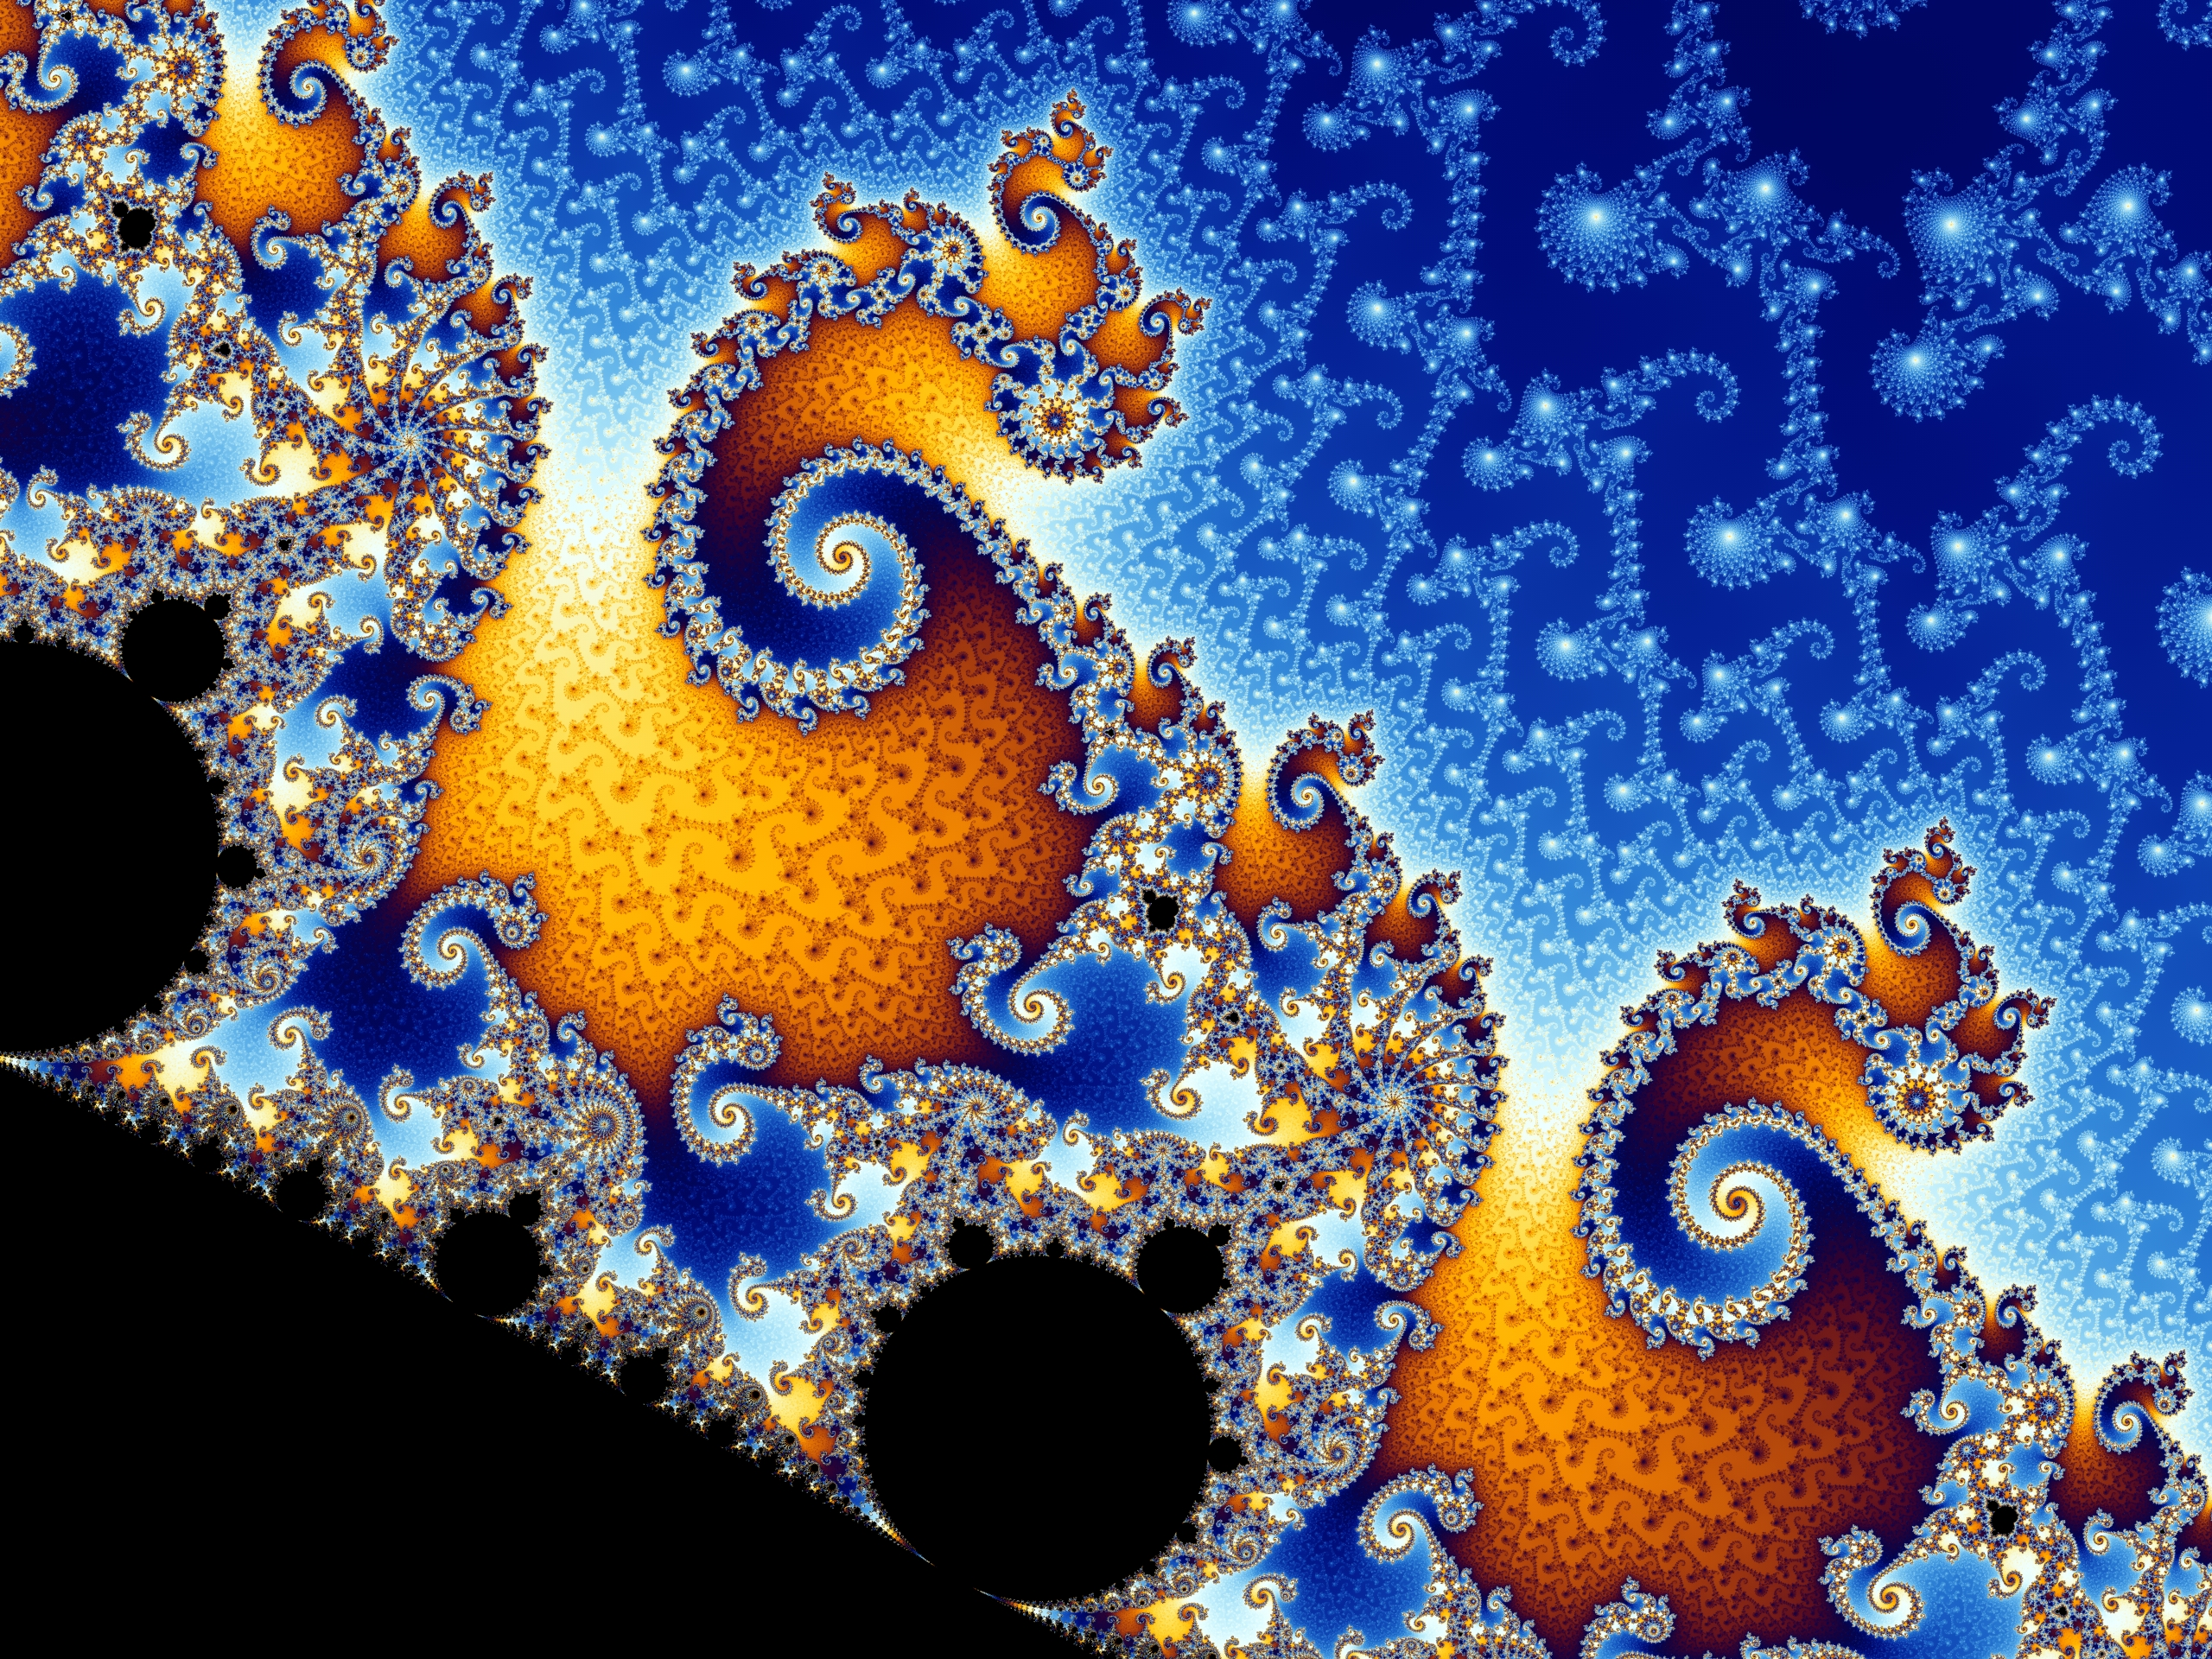
\includegraphics[width=0.30\textwidth]{Mandelbrot.pdf}
\end{wrapfigure}

The Mandelbrot set is generated by sampling complex numbers and testing, for each point, whether repeatedly iterating a simple mathematical function causes the values to diverge to infinity. By interpreting the real and imaginary parts of each number as image coordinates, pixels are colored according to how quickly their sequences diverge, while points that never diverge are shown in black. The resulting image reveals an intricate boundary that unfolds into endlessly finer, self-similar patterns under magnification. Despite its visual richness, the Mandelbrot set has very low Kolmogorov complexity, as it arises from an extremely short algorithm, illustrating how simple rules can produce extraordinary complexity in appearance while remaining simple in description.

\subsubsection* {Terra Australis Incognita}

\begin{wrapfigure}{L}{0.3\textwidth}
\centering
\includegraphics[width=0.30\textwidth]{terra_incognita.pdf}
\end{wrapfigure}

This antique map depicts a vast southern landmass labeled Terra Australis Incognita, the unknown southern land, a hypothetical continent once believed to balance the known continents of the Northern Hemisphere. Cartographers filled its empty expanse with speculative coastlines and imagined regions, a testament to how human minds try to complete what they do not yet understand. This map stands as a powerful allegory of the unknown: the regions of knowledge we do not even realize we are missing. Like explorers staring at blank spaces on their charts, we must first recognize that these voids exist before we can begin to illuminate them.

\subsubsection* {The School of Athens}

\begin{wrapfigure}{L}{0.3\textwidth}
\centering
\includegraphics[width=0.30\textwidth]{School_of_Athens.pdf}
\end{wrapfigure}

This fresco, The School of Athens by Raphael, portrays an idealized gathering of the great thinkers of classical antiquity (Plato, Aristotle, Socrates, Pythagoras, Euclid, and many others) engaged in animated debate and shared inquiry. Painted on the walls of the Vatican in the early 16th century, it celebrates the collective pursuit of wisdom through dialogue, reasoning, and teaching. The scene embodies the essence of learning as a cumulative human endeavor: knowledge grows not in isolation, but through the exchange of ideas across generations. It symbolizes the collaborative effort to diminish ignorance, as each mind contributes a fragment of understanding to the expanding edifice of human knowledge.

\subsubsection* {Ouroboros}

\begin{wrapfigure}{L}{0.3\textwidth}
\centering
\includegraphics[width=0.30\textwidth]{ouroboros.pdf}
\end{wrapfigure}

The Ouroboros, an ancient symbol depicting a serpent devouring its own tail, represents the eternal cycle of destruction and creation, of endings becoming beginnings. Often associated with alchemy, philosophy, and mysticism, it embodies the self-renewing nature of knowledge, how each resolution gives rise to new questions, and each discovery reshapes what remains unknown. The Ouroboros serves as a powerful metaphor for the dynamic process of inquiry: as we consume the known, we expose the unknown beyond it, endlessly renewing the pursuit of understanding.

\subsubsection* {Gutenberg's Printing Press}

\begin{wrapfigure}{L}{0.3\textwidth}
\centering
\includegraphics[width=0.30\textwidth]{gutenberg.pdf}
\end{wrapfigure}

The Gutenberg printing press, invented by Johannes Gutenberg in the mid-15th century, revolutionized the production and dissemination of knowledge. By introducing movable type and mechanical printing, Gutenberg transformed books from rare, hand-copied artifacts into mass-produced vehicles of ideas, enabling knowledge to spread across continents and generations. This invention ignited an unprecedented expansion of learning, accelerating the scientific revolution and reshaping human thought. The printing press symbolizes a turning point where the known began to outpace the unknown, an enduring reminder that advances in how we transmit knowledge can profoundly accelerate our conquest of ignorance.

\subsubsection* {Great Library of Alexandria}

\begin{wrapfigure}{L}{0.3\textwidth}
\centering
\includegraphics[width=0.30\textwidth]{Library_Alexandria.pdf}
\end{wrapfigure}

The Great Library of Alexandria, founded in the 3rd century BCE in ancient Egypt, was one of the most ambitious centers of learning in human history. It is said to have housed hundreds of thousands of scrolls, gathering the accumulated knowledge of the known world under one roof. Though ultimately destroyed, its legend endures as a symbol of humanity's longing to preserve and unify all understanding. The Library of Alexandria represents both the grandeur and fragility of our efforts to conquer ignorance, an eternal reminder that the pursuit of knowledge is vast, precious, and always vulnerable to loss.

\newpage

\subsubsection* {Tree of Knowledge}

\begin{wrapfigure}{L}{0.3\textwidth}
\centering
\includegraphics[width=0.30\textwidth]{tree_of_knowledge.pdf}
\end{wrapfigure}

The Tree of Knowledge has appeared in many cultural, religious, and philosophical traditions as a symbol of the branching structure of human understanding. From medieval "arbores scientiarum" to moral trees and the Kabbalistic "Etz Chaim", such diagrams attempt to organize all domains of thought as growing from shared roots and unfolding into diverse branches. They express the idea that knowledge is not a collection of isolated facts, but an interconnected living system where new ideas grow from older ones. The Tree of Knowledge embodies humanity's ongoing effort to map the known while hinting at the vast, unseen forest of the unknown that still lies beyond its outermost branches.






